\documentclass[../main.tex]{subfiles} 
\usepackage{ctex}
\usepackage{xltxtra}
\usepackage{graphicx}
\usepackage{booktabs}
\usepackage{amsmath}
\usepackage{mathdots}
\usepackage{amssymb}
\usepackage{cite}
\usepackage{appendix}
\usepackage{array}
\usepackage{subfigure}
\usepackage{multirow}
\begin{document}

    \subsection{模型导入}
    
        SVC:从sklearn.svm导入SVC

        Decision Tree:从sklearn.tree导入DecisionTreeClassifier

        Naive Bayes:从sklearn.naive\_bayes导入GaussianNB

        KNN:从sklearn.neighbors导入KNeighborsClassifier

        Random Forest:从sklearn.ensemble导入RandomForestClassifier

        CatBoost:从catboost导入CatBoostClassifier

    \subsection{训练集与测试集划分}

        由于官方测试集没有标签,只能将模型对于官方测试集的预测结果提交到Kaggle上进行测试并排行。所以在训练过程中只能对训练集进行重新划分出训练集和测试集,并且采用了k折交叉验证进行划分,此时每次迭代过程中每个样本只有一次被划入训练集或测试集的机会,避免了样本重复抽样的问题。
        
        对于k值的选定,若增大k值,在每次迭代过程中将会有更多的数据用于模型训练,能够得到最小偏差,同时算法时间延长。且训练块间高度相似,导致评价结果方差较高;
        若减小k值,降低模型在不同的数据块上进行重复拟合的性能评估的计算成本,在平均性能的基础上获得模型的准确评估。

        基于上述原则,最终确定了k值为10,此时训练集和测试集中的数据数量如图33所示。

        \begin{figure}[H]
            \centering
            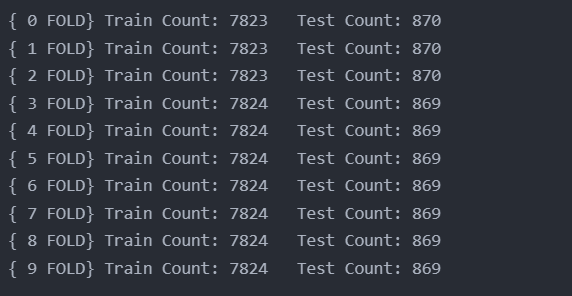
\includegraphics[scale=0.5]{Sec6_1.png}
            \caption{10折交叉验证}
        \end{figure}

    \subsection{模型参数设置}

        利用sklearn.model\_selection中的GridSearchCV函数对于每个模型设置了多种参数进行训练,如表5所示。并根据模型在测试集上的测试结果,选出最好的参数,进行模型评估。

        对于SVC,正如之前分析所说,不同的核函数会有不同的效果,因此选用线性核和高斯核分别进行尝试,而不同的惩罚因子C所允许的犯错大小也是不同的,因此对C也进行了测试。

        对于Decision Tree,主要调整的是树的深度和criterion,对于Max\_depth进行了不同值的考虑。

        对于Naive Bayes,主要测试的是var\_smoothing参数,主要防止的是有些特征出现方差为0的情况。

        对于KNN,主要调整的是n\_neighbors和p两个参数,分别指的是邻居的个数和距离度量公式。

        对于Random Forest,主要调整的是基学习器数量和最大深度。

        对于CatBoost,同样调整的是基学习器数量和最大深度以及学习率大小。

        \begin{table}[H]
            \centering
            \small
            \begin{tabular}{|c|cc|c|}
            \hline
            \multirow{2}{*}{\textbf{Model}}         & \multicolumn{2}{c|}{\textbf{Parameter}}                             & \multirow{2}{*}{\textbf{Best Parameter}} \\ \cline{2-3}
                                                    & \multicolumn{1}{c|}{\textbf{name}}  & \textbf{data}                 &                                          \\ \hline
            \multirow{2}{*}{\textbf{SVC}}           & \multicolumn{1}{c|}{C}              & 0.25, 0.5, 0.75, 1, 1.25, 1.5 & 1.5                                      \\ \cline{2-4} 
                                                    & \multicolumn{1}{c|}{kernel}         & 'linear', 'rbf'               & rbf                                      \\ \hline
            \multirow{2}{*}{\textbf{Decision Tree}} & \multicolumn{1}{c|}{max\_depth}     & 5,7,9,11                      & 7                                        \\ \cline{2-4} 
                                                    & \multicolumn{1}{c|}{criterion}      & 'gini','entropy'              &                                          \\ \hline
            \textbf{Naive Bayes}                    & \multicolumn{1}{c|}{var\_smoothing} & 1e-10, 1e-9, 1e-8, 1e-7       & 1e-07                                    \\ \hline
            \multirow{2}{*}{\textbf{KNN}}           & \multicolumn{1}{c|}{n\_neighbors}   & 3, 5, 7, 9                    & 9                                        \\ \cline{2-4} 
                                                    & \multicolumn{1}{c|}{p}              & 1, 2                          & 2                                        \\ \hline
            \multirow{2}{*}{\textbf{Random Forest}} & \multicolumn{1}{c|}{n\_estimators}  & 50, 100, 150, 200, 250, 300   & 100                                      \\ \cline{2-4} 
                                                    & \multicolumn{1}{c|}{max\_depth}     & 4, 6, 8, 10, 12               & 12                                       \\ \hline
            \multirow{3}{*}{\textbf{CatBoost}}      & \multicolumn{1}{c|}{learning\_rate} & 0.05, 0.1, 0.15               & 0.05                                     \\ \cline{2-4} 
                                                    & \multicolumn{1}{c|}{max\_depth}     & 4,8,12                        & 8                                        \\ \cline{2-4} 
                                                    & \multicolumn{1}{c|}{n\_estimators}  & 50, 100, 150, 200             & 200                                      \\ \hline
            \end{tabular}
        \end{table}

\end{document}